\documentclass[aspectratio=169]{beamer}
\usepackage[utf8]{inputenc}
\usepackage[T1]{fontenc}
\usepackage[brazil]{babel}
\usepackage{ragged2e}
\usepackage{booktabs}
\usepackage{verbatim}
\usepackage{gensymb}
\usepackage{multirow}
\usepackage{xcolor,colortbl}
\definecolor{verde}{rgb}{0,0.5,0}
\usepackage{listings}

\lstset{language=C++,
	backgroundcolor=\color{green!10},
	basicstyle=\ttfamily,
	keywordstyle=\color{blue}\ttfamily,
	stringstyle=\color{red}\ttfamily,
	commentstyle=\color{green}\ttfamily,
	morecomment=[l][\color{magenta}]{\#},
	extendedchars=true,
	showspaces=false,
	showstringspaces=false,
	%  numbers=left,
	%  numberstyle=\tiny,
	breaklines=true,
	backgroundcolor=\color{green!10},
	breakautoindent=true,
	captionpos=b,
	xleftmargin=0pt,
	literate=
	{á}{{\'a}}1
	{à}{{\`a}}1
	{ã}{{\~a}}1
	{â}{{\^a}}1
	{é}{{\'e}}1
	{ê}{{\^e}}1
	{í}{{\'i}}1
	{ó}{{\'o}}1
	{õ}{{\~o}}1
	{ú}{{\'u}}1
	{ü}{{\"u}}1
	{ç}{{\c{c}}}1
	{Á}{{\'A}}1
	{À}{{\`A}}1
	{Ã}{{\~A}}1
	{Â}{{\^A}}1
	{É}{{\'E}}1
	{Ê}{{\^E}}1
	{Í}{{\'I}}1
	{Ó}{{\'O}}1
	{Õ}{{\~O}}1
	{Ú}{{\'U}}1
	{Ü}{{\"U}}1
	{Ç}{{\c{C}}}1
}

\newcommand\setItemnumber[1]{\setcounter{enumi}{\numexpr#1-1\relax}}

\usetheme{AnnArbor}
\usecolortheme{orchid}
\usefonttheme[onlymath]{serif}

\AtBeginSection[]{
  \begin{frame}
  \vfill
  \centering
  \begin{beamercolorbox}[sep=8pt,center,shadow=true,rounded=true]{title}
    \usebeamerfont{title}\insertsectionhead\par%
  \end{beamercolorbox}
  \vfill
  \end{frame}
}

\title[\sc{Polimorfismo}]{Polimorfismo}
\author[Roland Teodorowitsch]{Roland Teodorowitsch}
%\institute[LP2 - EC - PUCRS]{Laboratório de Programação II - Curso de Engenharia de Computação - PUCRS}
\institute[POO - EC - PUCRS]{Programação Orientada a Objetos - ECo - Curso de Engenharia de Computação - PUCRS}
\date{3 de junho de 2024}

\begin{document}
\justifying

%-------------------------------------------------------
\begin{frame}
	\titlepage
\end{frame}

%=======================================================
\section{Polimorfismo}

%-------------------------------------------------------
\begin{frame}\frametitle{Introdução}
\begin{itemize}
	\item Observe a seguinte modelagem, em especial o método \texttt{double obtemSalario()}
\begin{figure}[h]
	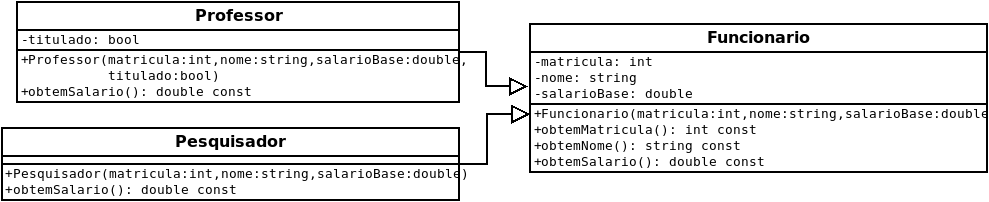
\includegraphics[height=0.33\paperheight]{pucrs-ec-poo-unidade_14-polimorfismo-laminas-funcionario.png}\\
\end{figure}
\end{itemize}
\end{frame}

%-------------------------------------------------------
\begin{frame}[fragile]\frametitle{Arquivo \texttt{Funcionario.hpp}}
\lstinputlisting[basicstyle=\ttfamily\scriptsize]{src/Funcionario/Funcionario.hpp}
\end{frame}

%-------------------------------------------------------
\begin{frame}[fragile]\frametitle{Arquivo \texttt{Funcionario.cpp}}
\lstinputlisting[basicstyle=\ttfamily\tiny]{src/Funcionario/Funcionario.cpp}
\end{frame}

%-------------------------------------------------------
\begin{frame}[fragile]\frametitle{Arquivo \texttt{Professor.hpp}}
\lstinputlisting[basicstyle=\ttfamily\scriptsize]{src/Funcionario/Professor.hpp}
\end{frame}

%-------------------------------------------------------
\begin{frame}[fragile]\frametitle{Arquivo \texttt{Professor.cpp}}
\lstinputlisting[basicstyle=\ttfamily\scriptsize]{src/Funcionario/Professor.cpp}
\end{frame}

%-------------------------------------------------------
\begin{frame}[fragile]\frametitle{Arquivo \texttt{Pesquisador.hpp}}
\lstinputlisting[basicstyle=\ttfamily\scriptsize]{src/Funcionario/Pesquisador.hpp}
\end{frame}

%-------------------------------------------------------
\begin{frame}[fragile]\frametitle{Arquivo \texttt{Pesquisador.cpp}}
\lstinputlisting[basicstyle=\ttfamily\scriptsize]{src/Funcionario/Pesquisador.cpp}
\end{frame}

%-------------------------------------------------------
\begin{frame}[fragile]\frametitle{Arquivo \texttt{main.cpp}}
\lstinputlisting[basicstyle=\ttfamily\tiny]{src/Funcionario/main.cpp}
\end{frame}

%-------------------------------------------------------
\begin{frame}\frametitle{Funções Virtuais}
\begin{itemize}
	\item Normalmente, o tipo do ponteiro define o método que será acionado
	\item \textbf{Polimorfismo} é a característica única de linguagens orientadas a objetos que permite que diferentes objetos comportem-se de diversas formas, dependendo do contexto
	\item Em C++ polimorfismo é obtido através de \textbf{funções virtuais}
	\item Funções virtuais são declaradas através da palavra reservada \texttt{virtual}
	\item É possível fazer redefinição de métodos em uma hierarquia
\end{itemize}
\end{frame}

%-------------------------------------------------------
\begin{frame}[fragile]\frametitle{Relembrando o Conceito de Herança...}
\begin{itemize}
	\item Utiliza-se objetos em hierarquia de classes:
\begin{columns}
\begin{column}{0.5\linewidth}
\lstinputlisting[firstline=1,lastline=9]{src/exemplo1.cpp}
\end{column}
\begin{column}{0.5\linewidth}
\begin{itemize}
	\item Como a classe \texttt{Derivada} é derivada da classe \texttt{Base}, todos os membros de \texttt{Base} também estarão em \texttt{Derivada}
	\item \texttt{Derivada} é um super-conjunto de \texttt{Base}: todas operações que podem ser feitas com objetos de \texttt{Base} também o podem com objetos de \texttt{Derivada}
	\item Um objeto da classe \texttt{Derivada} também é um objeto da classe \texttt{Base}
\end{itemize}
\end{column}
\end{columns}
\end{itemize}
\end{frame}

%-------------------------------------------------------
\begin{frame}[fragile]\frametitle{O Que Pode e o Que NÃO Pode Ser Feito?}
\lstinputlisting[basicstyle=\ttfamily\tiny]{src/exemplo1.cpp}
\end{frame}

%-------------------------------------------------------
\begin{frame}[fragile]\frametitle{Explorando Polimorfismo na Classe \texttt{Funcionario}}
\begin{itemize}
\item Alterando a classe \texttt{Funcionario}:
\lstinputlisting[basicstyle=\ttfamily\tiny]{src/Funcionario2/Funcionario.hpp}
\end{itemize}
\end{frame}

%-------------------------------------------------------
\begin{frame}[fragile]\frametitle{Explorando Polimorfismo com uma Nova \texttt{main()} (2)}
\begin{itemize}
\item Agora o que define a versão de \texttt{obtemSalario()} é o tipo de objeto e não mais o ponteiro:
\lstinputlisting[basicstyle=\ttfamily\tiny]{src/Funcionario2/main.cpp}
\end{itemize}
\end{frame}

%-------------------------------------------------------
\begin{frame}[fragile]\frametitle{Classes Virtuais Puras}
\begin{itemize}
\item Em C++, é possível definir classes que nunca serão instanciadas, definindo somente a sua interface, que deverá ser implementada nas suas classes derivadas
\item Isso é feito declarando métodos virtuais puros (o médodo é declarado com \texttt{virtual} e acrescenta-se \texttt{= 0;} na sua declaração):
\lstinputlisting[basicstyle=\ttfamily\tiny]{src/exemplo2.cpp}
\end{itemize}
\end{frame}

%=======================================================
\section{Lista de Exercícios}

%-------------------------------------------------------
\begin{frame}[fragile]\frametitle{Exercício 1}
\begin{enumerate}
	\setItemnumber{1}
	\item Execute os seguintes passos:
	\begin{itemize}
		\item Crie uma classe abstrata chamada \texttt{Animal} que armazene o nome e a idade de um animal (informados via método construtor)
		\item Defina métodos de acesso para os atributos nome e idade
		\item Defina um método (virtual) chamado \texttt{string emiteSom()} -- o objetivo deste método, nas classes derivadas, é retornar um string com o som emitido pelo animal (por exemplo: ``au au'', ``piu piu'', etc.)
		\item Escreva pelo menos 3 classes derivadas de \texttt{Animal}, definindo pelo menos 3 tipos de animais diferentes
		\item Escreva um programa (\texttt{main()}) que instancia um vetor de 6 animais, instanciando 2 animais de cada tipo criado (	imagine uma jaula em um zoológico com esses animais)
		\item Após, usando um comando \texttt{for}, imprima nome e a idade do animal armazenado na jaula, bem como o som emitido por cada animal
	\end{itemize}
\end{enumerate}
\end{frame}

%-------------------------------------------------------
\begin{frame}[fragile]\frametitle{Exercício 2}
\begin{enumerate}
	\setItemnumber{2}
	\item Um banco trabalha com três tipos de contas:
	\begin{itemize}
		\item conta corrente comum (classe \texttt{ContaComum});
		\item conta corrente com limite (classe \texttt{ContaLimite});
		\item conta poupança (classe \texttt{ContaPoupanca}).
	\end{itemize}
	Em todos os casos é necessário guardar o número da conta, o nome do correntista e o saldo. Para a conta poupança é necessário guardar o dia do aniversário da conta (quando são creditados os juros). Já para a conta com limite é necessário guardar o valor do limite. As contas também armazenam uma lista de transações (até 10 transações). Uma transação é definida por uma data, valor da transação e descrição. Se o valor for negativo, a transação é considerada um débito (crédito caso contrário).\\
	Para obter a data em uma \texttt{string}, você pode utilizar as linhas abaixo:
\begin{lstlisting}[language=C++,basicstyle=\ttfamily\scriptsize]
#include <ctime>
time_t now = time(0);
string date = ctime(&now);
\end{lstlisting}
\end{enumerate}
\end{frame}

%-------------------------------------------------------
\begin{frame}[fragile]\frametitle{Exercício 2}
\begin{enumerate}
	\setItemnumber{2}
	\item (Continuação)\\
	As operações possíveis são:
	\begin{itemize}
		\item depósito;
		\item saque;
		\item impressão de extrato.
	\end{itemize}
	Essas operações devem ser definidas numa classe abstrata pura (interface) denominada \texttt{Conta}. A operação de depósito é igual nos três tipos de conta. O saque só é diferente na conta com limite, pois esta admite que o saldo fique negativo até o limite estabelecido.\\
	Finalmente o extrato é diferente para as três:
	\begin{itemize}
		\item na conta comum exibe o número da conta, nome do cliente, transações e o saldo;
		\item na conta limite imprime também o valor do limite;
		\item na conta poupança imprime também o dia do aniversário.
	\end{itemize}
\end{enumerate}
\end{frame}

%-------------------------------------------------------
\begin{frame}[fragile]\frametitle{Exercício 2}
\begin{enumerate}
	\setItemnumber{2}
	\item (Continuação)\\
	Implemente a hierarquia de classes das contas explorando \textbf{polimorfismo}.\\
	Ao final, escreva um programa em C++ que permita ao usuário fazer depósitos, saques e verificação de extrato nas suas contas a partir do número da conta. Utilize um único vetor para armazenar todos os tipos de contas.
\end{enumerate}
\end{frame}

%=======================================================
\section{Créditos}

%-------------------------------------------------------
\begin{frame}\frametitle{Créditos}
\begin{itemize}	
	\item Estas lâminas contêm trechos de materiais disponibilizados pelos professores Rafael Garibotti, Matheus Trevisan, Daniel Callegari, Sandro Fiorini e Bernardo Copstein.
\end{itemize}
\end{frame}

%=======================================================
\section{Solução dos Exercícios}

%-------------------------------------------------------
\begin{frame}\frametitle{Exercício 1: \texttt{exercicio1.cpp}}
\fontsize{3pt}{5pt}\selectfont{
\lstinputlisting{src/exercicio1.cpp}
}
\end{frame}

%-------------------------------------------------------
\end{document}

